\documentclass[varwidth=true, border=2pt]{standalone}

\usepackage{pgfplots}
\usepackage{tikz}

\begin{document}
		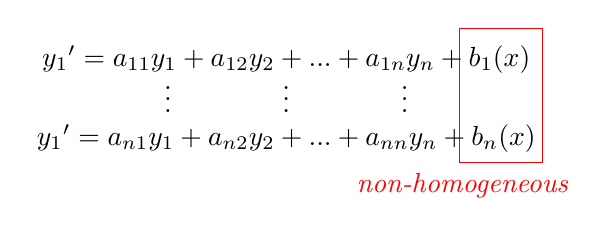
\begin{tikzpicture}
		\draw[red] (2.2,0.7) -- (3.25,0.7) -- (3.25,2.4) -- (2.2,2.4) -- (2.2,0.7);
		\node (E1) at (0,2) {$y_1 \,\! ^\prime = a_{11}y_1 + a_{12}y_2 + ... + a_{1n}y_n + b_1(x)$};
		\node (D) at (0, 1.6){$\vdots \qquad \qquad \vdots \qquad \qquad \vdots$};
		\node (E2) at (0,1) {$y_1 \,\! ^\prime = a_{n1}y_1 + a_{n2}y_2 + ... + a_{nn}y_n + b_n(x)$};
		\node(N) [red] at (2.25, 0.4){\textit{non-homogeneous}};
		\end{tikzpicture}
\end{document}